\aufgabenteil{a)}
Die Idee hinter der Code-Generierung ist, durch das automatisierte Generieren von Programmcode(teilen) aus
einer Modellsprache sowohl Zeit einzusparen als auch eine höhere Qualität in Hinblick auf die Strukturierung und Lesbarkeit zu erzielen.

\aufgabenteil{b)}
%%%%%%%%%%%%%%%%%%%%%%%%%%%%%%%%%%%%%%%%
%% Klassendiagramm, evtl. texen       %%

\begin{figure}[h]
  \centering
  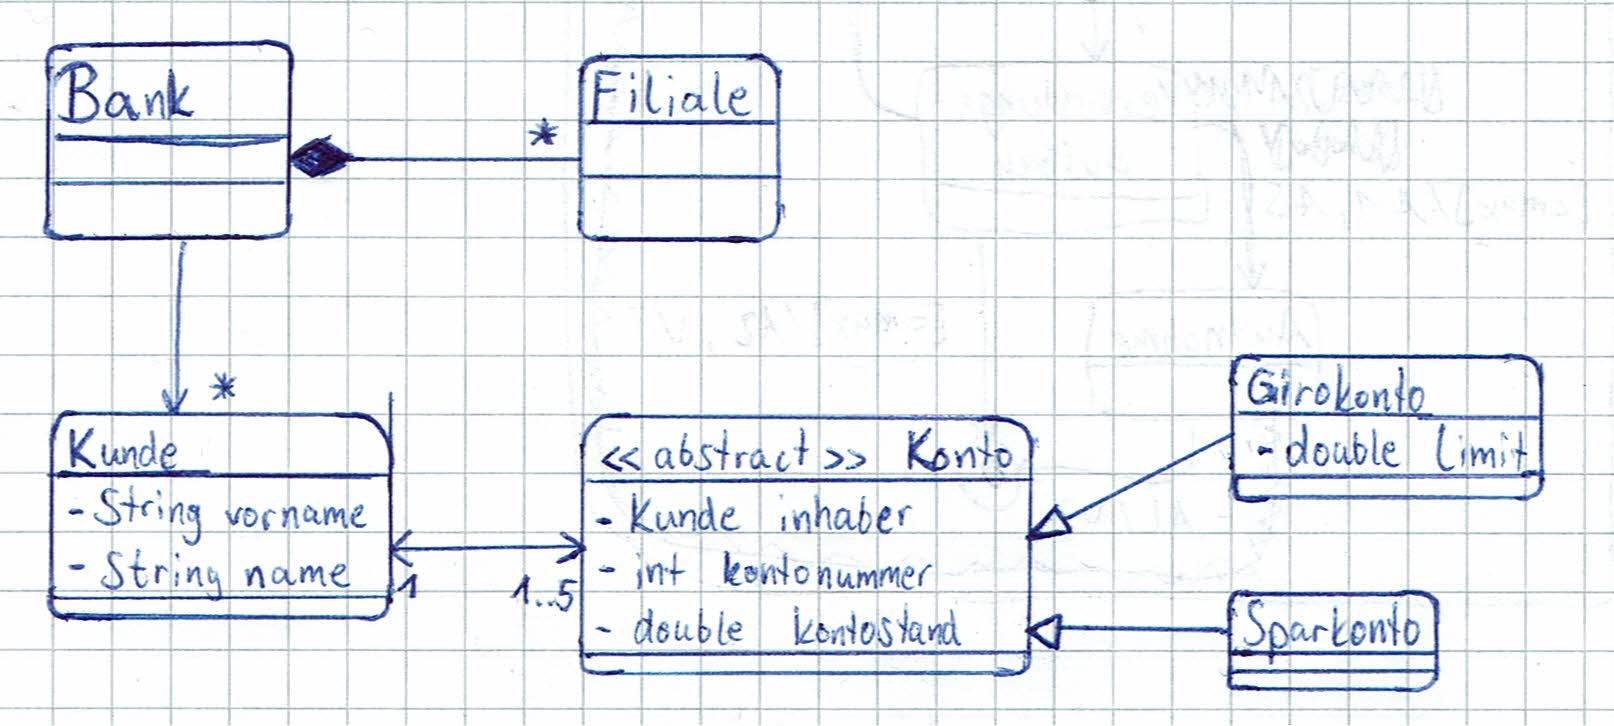
\includegraphics{3b_classdiag}
\end{figure}

%%                                    %%
%%%%%%%%%%%%%%%%%%%%%%%%%%%%%%%%%%%%%%%%

\lstset{
    %basicstyle=\ttfamily,
    keywordstyle=\bfseries,
    showstringspaces=false,
    morekeywords={classdiagram, class, abstract, extends, association}
}
\begin{minipage}{\linewidth}
Nun folgt die textuelle Beschreibung der geforderten Elemente des Klassendiagramms:\\
\begin{lstlisting}
classdiagram BankSystem {
    class Kunde {
       String vorname;
       String name;
    }
    abstract class Konto {
       Kunde inhaber;
       int kontonummer;
       double kontostand;
    }
    class Girokonto extends Konto {
       double limit;
    }
    association [1] Kunde <-> Konto [1..5];
}
\end{lstlisting}
\end{minipage}